\section{LP Duality, Matrix Games, and Integer linear programming.}
\subsection{Dual}
\begin{itemize}
	\item Et lineært programmerings problem i standard form (\textbf{primal problemet})
  \begin{alignat*}{2}
    \text{max} \quad  & \sum_{j=1}^n c_jx_j && \\
    \text{s.t.} \quad & \sum_{j=1}^n a_{ij}x_j \leq b_i && \quad i = 1,2,\dots,m \\
    & x_j \geq 0 && \quad j = 1,2, \dots, n
  \end{alignat*}
  har følgende \textbf{dual lineær program}
  \begin{alignat*}{2}
    \text{min} \quad  & \sum_{i=1}^m b_iy_i && \\
    \text{s.t.} \quad & \sum_{i=1}^m a_{ij}y_i \geq c_i && \quad j = 1,2,\dots,n \\
    & y_i \geq 0 && \quad i = 1,2, \dots, m
  \end{alignat*}
  \item Hvis tager dual to gange får man primal tilbage
  \item \textbf{Weak Duality Theorem}  Hvis $(x_1, x_2, \dots, x_n)$ er feasible for primal og $(y_1, y_2, \dots, y_n)$ er feasible for dualen så
  \begin{equation*}
    \sum_j c_jx_j \leq \sum_i b_iy_i 
  \end{equation*}
  \begin{proof} 
    Beviset følger af følgende uligheder 
    \begin{align*}
      \sum_j c_jx_j &\leq \sum_j \bigg(\sum_i y_i a_{ij}\bigg) x_j \\
                   &= \sum_{ij} y_ia_{ij} x_j \\
                   &= \sum_i (\sum_j a_{ij} x_j) y_i \\
                   &\leq \sum_i b_i y_i
    \end{align*}
    Den første ulighed følger af $x_j$ ikke er negativ og alle $c_j$ ikke er større end $\sum_i y_ia_{ij}$. Den anden ulighed følger af ligende grunde

  \end{proof}
\end{itemize}

\begin{itemize}
  \item \textbf{Strong Duality Theorem} Hvis primal problemet har en optimal løsning:
  \begin{equation*}
    x^*= (x_1^*, x_2^*, \dots, x_n^*)
  \end{equation*}	
  så har den dual en optimal løsning
  \begin{equation*}
    y^*= (y_1^*, y_2^*, \dots, y_n^*)
  \end{equation*}	
  således at	
  \begin{equation*}
    \sum_j c_j x_j^* = \sum_i b_i y_i^*
  \end{equation*}	
  Dette følger at den dual dictionary altid er den negative transpose af primal (Se Figur \ref{fig:pivot})  
  \begin{figure}[ht]
    \centering
    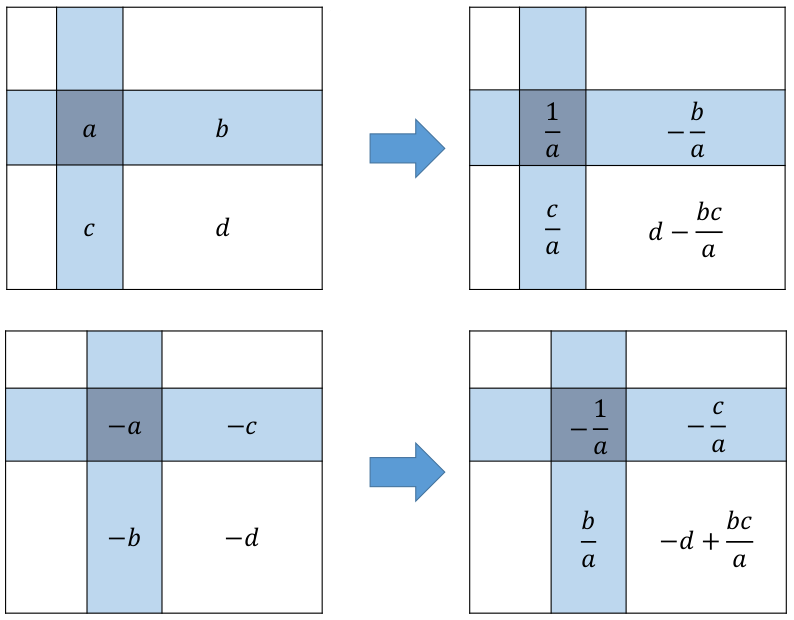
\includegraphics[width=300px]{img/pivot}
    \caption{Abstrakt beskrivelse af pivoting\label{fig:pivot}}
  \end{figure}

  \item Hvis primal problemet er unbounded så er dual problemet infeasible
  \begin{itemize}
  	\item Hvis dual problemet er unbounded så er primal problem infeasible
  \end{itemize}
  \item For et generalt lineært programmerings problem holder følgende regler for at tage duelen
  \begin{table}[H]
    \centering
    \begin{tabular}{l|l}
    Primal (Maksimering) & Dual (Minimering) \\ \hline
    $\leq$ for restrektion & $\geq 0$ for variable  \\
    $\geq$ for restrektion & $\leq 0$ for variable  \\
    $=$ for restrektion & fri variable  \\ \hline
    $\geq 0$ for restrektion & $\geq$ for restrektion \\
    $\leq 0$ for restrektion & $\leq$ for restrektion \\
    fri variable & $=$ for restrektion  \\
    \end{tabular}
  \end{table}
\end{itemize}

\begin{itemize}
	\item \textbf{Complementary Slackness Egenskaben} Løsninger $x$ and $y$ til henholdsvis en primal og en overholder
  \begin{itemize}
  	\item For alle $i=1,2,\dots,m$ mindst en af følgende holder:
    \begin{enumerate}
    	\item $\sum_{j=1}^na_{ij}x_j=b_i$ \quad (den i'te primal restrektion har slack $0$)
      \item $y_i=0$ \hspace{50pt} (den i'te dual variable er $0$)
    \end{enumerate}
  	\item For alle $j=1,2,\dots,n$ mindst en af følgende holder:
    \begin{enumerate}
    	\item $\sum_{i=1}^ma_{ij}y_i=c_j$ \quad (den j'te dual restrektion har slack $0$)
      \item $x_i=0$ \hspace{50pt} (den j'te primal variable er $0$)
    \end{enumerate}
  \end{itemize}
  \item \textbf{Complementary Slackness Theorem} Hvis $x$ og $y$ er feasible løsninger til $P$ og $D$. Så er $x$ og $y$ begge optimal hvis og kun hvis $x$ og $y$ overholder Complementary Slackness Egenskaben
  \begin{proof} 
    Hvis man kigger på ulighederne brugt til at bevise Weak Duality Theorem:
    \begin{equation*}
      \sum_j c_jx_j \leq \sum_j \bigg(\sum_i y_i a_{ij}\bigg) x_j = \sum_{ij} y_ia_{ij} x_j = \sum_i (\sum_j a_{ij} x_j) y_i \leq \sum_i b_i y_i
    \end{equation*}
     være ligheder. Den sidste ulighed bruges til at bevise theoremet:
    \begin{equation*}
      \sum_i (\sum_j a_{ij} x_j) y_i = \sum_i b_i y_i \Leftrightarrow \sum_i (\sum_j a_{ij} x_j - b_i) y_i = 0
    \end{equation*}
    $a_{ij} x_j - b_i$ for alle $i,j$ er positiv, da løsningen er feasible. Dermed må enten $a_{ij} x_j - b_i=0$ eller $y_i=0$ for alle termer, da de to udtryk der bliver multipliceret ikke må være negative. Dermed gælder den første del af theoremet, den anden kan bevises på samme måde ved at bruge den første lighed.     
  
  \end{proof}
  \item \textbf{Farkas Lemma} Systemet $Ax \leq b$ har ingen løsninger hvis og kun hvis der eksisterer et $y$ således at $A^T y = 0$ hvor det gælder at $y \geq 0$ og $b^T y <0$
  \item \textbf{Strict complementary slackness egenskaben} Løsninger $x$ og $y$ overholder følgende
  \begin{itemize}
  	\item For alle $i=1,2,\dots,m$ \textbf{præcis} en af følgende holder:
    \begin{enumerate}
    	\item $\sum_{j=1}^na_{ij}x_j=b_i$ \quad (den i'te primal restrektion har slack $0$)
      \item $y_i=0$ \hspace{50pt} (den i'te dual variable er $0$)
    \end{enumerate}
  	\item For alle $j=1,2,\dots,n$ \textbf{præcis} en af følgende holder:
    \begin{enumerate}
    	\item $\sum_{i=1}^ma_{ij}y_i=c_j$ \quad (den j'te dual restrektion har slack $0$)
      \item $x_i=0$ \hspace{50pt} (den j'te primal variable er $0$)
    \end{enumerate}
  \end{itemize}
  \item \textbf{Strict complementary slackness theorem} Hvis er primal problem har en optimal løsning, så eksisterer der optimale løsninger $x$ til primal and $y$ til dual der overholder complementary slackness egenskaben \\
\end{itemize}

\subsection{Matrix spil}
\begin{itemize}
	\item Et \textbf{matrix game} er et to persons spil defineret på følgende måde
  \begin{itemize}
    \item Et spil er defineret ud fra en \textbf{payout matrix} $A \in \text{Mat}_{(n,m)}(\R)$
    \item Et matrix game foregår på følgende måde, hvor spillerne kender $A$ 
    \item Rækkespilleren (Minnie) vælger et valg $i \in \{1,\dots,n\}$  
    \item Søjlespilleren (Max) vælger et valg $j \in \{1,\dots,m\}$  
    \item Minnie betaler $a_{ij}$ kroner til Max
    \item Matrix spil er nul sum spil, da Max får præcis det Minnie mister
    \item Et negativt tal bruges til at sende penge den modsatte vej
  \end{itemize}
  \item En \textbf{randomiseret strategi} er hvor hvert træk af spilleret virker tilfældig for den anden spiller ud fra en sandsynlighedsdistribution
  \begin{itemize}
    \item En vektor $y$ er en \textbf{stokastisk vektor}, hvis den består af sandsynligheder 
    \begin{itemize}
    	\item dvs. $y \geq 0$ og $e^Ty = 1$, hvor $e$ er vektoren med $e_i = 1$ for $i=1,\dots,n$    
    \end{itemize}
    \item Den stokastiske vektor $y$ er vektoren, hvor $y_i$ er sandsynligheden for at Minnie vælger action $i$ 
  	\item Den stokastiske vektor $x$ er vektoren, hvor $x_j$ er sandsynligheden for at Max vælger action $j$ 
    \item Den forventede payout for Max er 
    \begin{equation*}
      \sum_{i,j} y_ia_{ij}x_j = y^T A x
    \end{equation*}
  \end{itemize}
\end{itemize}

\begin{itemize}
  \item Den optimale strategi $x$ for Max kan findes ved at finde følgende maximum
  \begin{equation*}
    \max_x \ \min_y \ y^T A x
  \end{equation*}
  hvor $y$ og $x$ kun er over stokastiske vektorer  
  \begin{itemize}
    \item Den inderste optimering kan gøres over deterministisk strategier i stedet (Fundamental Theorem of Linear Programmering):
    \begin{equation*}
      \min_y y^T Ax = \min_i e_i^T Ax
    \end{equation*}
    \item Dermed kan problemet opskrives på følgende måde
    \begin{alignat*}{2}
      \max \quad  &  (\min_i e_i ^T A x) && \\
      \text{s.t.} \quad & \sum_{j=1}^n x_j = 1 && \\
      & x_j \geq 0 && \quad j=1,2,\dots,n
    \end{alignat*}
    \item Hvis en ny variable $v$ bliver introduceret, som repræsenterer en nedre grænse på $e_i^T Ax$ kan det omformuleres som et linært program
    \begin{alignat*}{2}
      \max \quad  & v && \\
      \text{s.t.} \quad &  v \leq e_i ^T A x && \quad  i = 1,2,\dots,m \\
      & \sum_{j=1}^n x_j = 1 && \\
      & x_j \geq 0 && \quad j=1,2,\dots,n
    \end{alignat*}
    \item Dette kan skrives i vektor notation på følgende måde :
    \begin{alignat*}{1}
      \max \quad  & v \\
      \text{s.t.} \quad &  ve-Ax \leq 0 \\
      & e^T x = 1 \\
      & x \geq 0
    \end{alignat*}
  \end{itemize}
  \item Den optimal strategi for Minnie kan findes på samme måde vha. følgende min-max problem 
  \begin{equation*}
    \min_y \ \max_x y^TAx
  \end{equation*}
  som kan omformuleres til følgende lineært programmeringsproblem 
  \begin{alignat*}{1}
    \min \quad  & u \\
    \text{s.t.} \quad &  ue-Ay \geq 0 \\
    & e^T y = 1 \\
    & y \geq 0
  \end{alignat*}
  \item \textbf{Minimax Theorem} Der eksisterer stokastiske vektorer $x^*$ og $y^*$ for hvilket 
  \begin{equation*}
    \max_x y^{*^T} Ax = \min_y y^T A x^*
  \end{equation*}
  \begin{proof} 
    Strong Duality Theoremet siden de to problemer er dual af hinanden. 
  \end{proof}
  \item Den fælles værdi $v^* = u^*$ kaldes for værdien af spillet 
  \begin{itemize}
  	\item Hvis et spil har en værdi på nul, er det et fair spil.
    \item Spil hvor de to spiller ombyttelig er fair
    \begin{itemize}
    	\item Bliver kaldt symmetriske 
      \item De har payoff matricer, hvor om det gælder at $a_{ij} = -a_{ji}$ for alle $i$ og $j$
    \end{itemize}
  \end{itemize} 
  \item \textbf{Principle of indifference} Givet optimal strategier $p^*$ for Max og $q^*$ for Minnie. Så er værdien den samme uanset hvilken række $q^*_i > 0$ Minnie vælger, hvis Max bruger $p^*$.
  \begin{proof} 
    Følger af Complementary Slackness Theoremet, da hvis $q_i^*>0$, så må den i'te restrektion være opfyldt med lighed 
  \end{proof}
  \item Hvis Minnie vælger en række, hvor $q_i^*=0$ for en optimal strategi $q^*$, findes der en optimal strategi $p^*$ som giver en større forventede værdi for Max
  \begin{proof} 
    Følger af Strict Complementary Slackness
  \end{proof}
  \item \textbf{Nash equilibrium} En par af randomiseret strategier $(x^*, y^*)$ er de bedste reaktioner til hinanden dvs. de svar der maksimerer deres forventede indtjeninger
  \item \textbf{Theorem} Et part af randomiseret strategier $(x^*,y^*)$ er et nash equilibrium hvis og kun hvis de begge er optimale
\end{itemize}

\subsection{Integer lineær programmering}
\begin{itemize}
	\item Integer lineær programmer er lineærer programmer, som også må have integer restrektioner dvs. programmer på følgende form:
   \begin{alignat*}{1}
    \min \quad  & c^Tx \\
    \text{s.t.} \quad &  Ax \leq b \\
    & x \geq 0 \\
    & x \in \mathbb Z^n
  \end{alignat*}
  \item De kan også have restrektioner, for hvilken mængde en del af variablerne er i 
  \item Det er ikke alle variabler der behøves at være integers
  \item De gør det muligt at udtrykke en lang række nye problemer så som TSP
  \item Problemet er NP komplet og derfor er det noget svære end standard lineær programmering
\end{itemize}

\subsubsection{The Traveling Salesman Problem}
\begin{itemize}
	\item Problemet er følgende:
  \begin{itemize}
  	\item En sælger skal besøge $n$ byer 
    \item Målet er at starte fra by $0$ besøge alle byer og komme tilbage til by $0$ igen
    \item Distancen mellem byerne er $c_{ij}$
    \item Han vil gerne minimere den totale distance
  \end{itemize}
  \item For at udtrykke problemet bruges følgende variabler og restrektioner:
  \begin{itemize}
  	\item For hver $(i,j)$ en decision variable $x_{ij}$ er introduceret, hvilket beskriver hvorvidt han besøger by $j$ lige efter by $i$
    \item Følgende restrektion sørger for at man kun kan gå fra en anden by fra en given by
    \begin{equation*}
      \sum_{j} x_{ij} = 1 \quad i=0,1,\dots,n-1
    \end{equation*}
    \item Følgende restrektion sørger for at man kun kan komme fra en by til en given by
    \begin{equation*}
      \sum_{i} x_{ij} = 1 \quad j=0,1,\dots,n-1
    \end{equation*}
    \item Lad $t_i$ for $i=0,1,\dots, n-1$ være defineret til at være det stop for hvilket by $i$ bliver besøgt
    \item For at sikre at turen bliver sammenhængende, skal en given $t_j$ overholde følgende restrektion:
    \begin{equation*}
      t_j \geq 
      \begin{cases}
        \mbox{$t_i+1-n$} & \mbox{hvis $x_{ij}= 0$} \\
        \mbox{$t_i+1$} & \mbox{hvis $x_{ij}= 1$} 
      \end{cases}
    \end{equation*}
    som kan blive skrevet ud således
    \begin{equation*}
      t_j \geq t_i +1 - n(1-x_{ij}) \quad i \geq 0, j \geq 1, i \neq j
    \end{equation*}
  \end{itemize}
  \item Problemet kan formueleret som følgende ILP:
  \begin{alignat*}{2}
         \min \quad  & \sum_{i,j=0}^{n-1}c_{ij}x_{ij} \\
   \text{s.t.} \quad & \sum_{j} x_{ij} = 1 &&\quad i=0,1,\dots,n-1 \\
                     & \sum_{i} x_{ij} = 1 &&\quad j=0,1,\dots,n-1 \\
                     & t_j \geq t_i +1 - n(1-x_{ij}) &&\quad i \geq 0, j \geq 1, i \neq j \\
                     & t_0 = 0 \\
                     & t_j \in \{0, \dots, n\} \\
                     & x_{ij} \in \{0,1\}
 \end{alignat*}
\end{itemize}

\subsubsection{Branch and Bound}
\begin{itemize}
	\item Branch and Bound er en algoritme, der bruges til at finde løsninger til ILP 
  \item LP relaxation af en ILP er det tilsvarende LP problem man får, hvis man fjerner integer restrektioner
  \item Lad $P^*$ være LP relaxationen af en ILP $P$ 
  \item Algoritmen kører på følgende måde
  \begin{enumerate}
  	\item Løs $P^*$ (fx. ved brug af Simplex algoritmen)
    \item Hvis $P^*$ er infeasible, så er $P$ infeasible (retuner (\textbf{null}, $-\infty$))
    \item Ellers lad $(x^*,\lambda^*)$ være den optimale løsning til $P^*$
    \item Hvis $x^*$ er integer, retuner $(x^*,\lambda^*)$
    \item Hvis $\lambda^* \leq$ currentBest(bound), retuner en branch uden løsning (retuner (\textbf{null}, $-\infty$))
    \item Ellers vælg et $i$ således at $x_i^* \notin \mathbb Z$
    \item Løs rekursivt (branch) ( $P^*[u_i := \lfloor x_i^* \rfloor$, currentbest) for at få $(x^l, \lambda^l)$
    \item Løs rekursivt (branch) ( $P^*[l_i := \lceil x_i^* \rceil$, currentbest) for at få $(x^r, \lambda^r)$
    \item Hvis $\lambda^l > \lambda^r$, retuner $(x^l, \lambda^l)$ ellers retuner $(x^r, \lambda^r)$
  \end{enumerate}
  \item Grunde til at dybde først er valgt
  \begin{enumerate}
  	\item Mange integer løsninger ligger dybt i træet, derfor finder man en løsning hurtigere som man kan bruge til at afvise nogle af de dårlige grene
    \item Det er nemmere at kode rekursivt
  \end{enumerate}

\end{itemize}

\newpage
%%% Local Variables:
%%% mode: latex
%%% TeX-master: "optimering-noter"
%%% End:
